\subsection{离散时间傅里叶变换}

\subsubsection{采样信号与采样频谱}

对于采样信号
\begin{align*}
    \hat{f}(t) = \sum_{n = -\infty}^{+\infty}f(nT_s)\delta(t - nT_s),
\end{align*}
以及其频谱函数
\begin{align*}
    \hat{F}(\omega) = \frac{1}{T_s}\sum_{k = -\infty}^{+\infty}F(\omega - k\omega_s),
\end{align*}
而言,如果采样过程满足采样定理的要求,则在奈奎斯特区间内,以下等式成立:
\begin{align*}
    T\hat{F}(\omega) = F(\omega), \quad \omega \in \left[-\frac{\omega_s}{2}, \frac{\omega_s}{2}\right].
\end{align*}
如果采样过程不满足采样定理的要求,则会发生混叠,在 $[-\omega_s/2, \omega_s/2]$ 这个
区间内混有其他部分``扩展''过来的密度分布。此时
\begin{align*}
    T\hat{F}(\omega) = F(\omega) + F(\omega - \omega_s) + F(\omega + \omega_s) + \cdots,
\end{align*}
我们可以认为,$F(\omega) \approx T\hat{F}(\omega)$。

\begin{theorem}
    对于连续时间信号 $f(t)$ 进行以 $T_s$ 为时间间隔的采样,得到序列 $f(nT_s)$,
    其中 $n \in \set{Z}$。那么,
    \begin{align*}
        \hat{F}(\omega) = \sum_{n = -\infty}^{+\infty}f(nT_s)\mathe^{-\mathi\omega nT_s}.
    \end{align*}
    这说明仅使用采样值 $f(nT_s)$ 即可计算出理想采样信号的频谱密度函数。
    注意,此时的频谱密度函数 $\hat{F}(\omega)$ 是连续的,且为周期函数。
\end{theorem}

\begin{theorem}
    若将 DTFT 看做是对 $\hat{F}(\omega)$ 的傅里叶展开,则 $f(nT_s)$ 即为
    $\hat{F}(\omega)$ 的傅里叶系数。因此,
    \begin{align*}
        f(nT_s) = \frac{1}{\omega_s}\int_{-\omega_s/2}^{\omega_s/2}\hat{F}(\omega)\mathe^{\mathi\omega nT_s}\D{\omega}.
    \end{align*}
\end{theorem}

\subsubsection{数字信号与数字频谱}

由于采样间隔为固定的值,因此不妨设 $T_s = 1$,这就是在对 DTFT 进行
频率归一化(采样间隔归一化等价于频率归一化,因为二者是互为倒数的)。
这样,具体的物理时间被抽象为了数字信号中一个无量纲的``单位时间''。

\begin{definition}[离散时间傅里叶变换]
    我们称时间间隔归一的离散信号序列为\bd{数字信号},
    称其 DTFT 频谱函数为\bd{数字频谱}。
    设 $x(n)$ 为数字信号,其\bd{离散时间傅里叶变换}(DTFT)为 $X(\omega)$,则
    \begin{align*}
        X(\omega) & = \DTFT{x(n)} = \sum_{n = -\infty}^{+\infty}x(n)\mathe^{-\mathi\omega n}.
    \end{align*}
    反之,若已知 $X(\omega)$,则可以通过\bd{逆离散时间傅里叶变换}(IDTFT)求得 $x(n)$:
    \begin{align*}
        x(n) & = \IDTFT{X(\omega)} = \frac{1}{2\pi}\int_{-\pi}^{\pi}X(\omega)\mathe^{\mathi\omega n}\D{\omega}.
    \end{align*}
\end{definition}

\begin{remark}
    对于实际信号(模拟信号)而言,CTFT 中得到的是模拟频率 $\Omega$。
    在 DTFT 引入归一化时间后,变换结果是数字频率 $\omega$。
    模拟频率的奈奎斯特区间是
    \begin{align*}
        \left[-\frac{\Omega_s}{2}, \frac{\Omega_s}{2}\right],
    \end{align*}
    其中 $\Omega_s = 2\pi/T_s$,而数字频率的奈奎斯特区间是 $[-\pi, \pi]$。

    数字频率和模拟频率之间的关系是
    \begin{align*}
        \omega = \Omega \cdot \frac{2\pi}{\Omega_s} = \Omega \cdot T_s = \frac{\Omega}{f_s}.
    \end{align*}
    即数字频率是模拟频率的 $1/f_s$ 倍。这可以看做是将 $\Omega$ 的取值范围
    从 $[-\Omega_s/2, \Omega_s/2]$ 缩放到 $[-\pi, \pi]$。
\end{remark}

\begin{remark}
    进行频率归一化有以下好处:
    \begin{enumerate}[label=(\arabic*)]
        \item 频谱函数主周期内的形状,如果不考虑高低变化的话,
            则形状与采样间隔无关。
        \item 采样频率归一化使频谱重复间隔也会统一成 $2\pi$。
            考虑到离散信号频谱总是周期的函数,所以研究时可以对
            采样信号的实际频谱的周期进行抽象化的处理。抽象为 $2\pi$ 是很方便的。
        \item 在计算机程序中,计算过程可以只考虑数值表示,而不用考虑信号样本间的
            真实时间间隔。从算法效果上看,这不仅不会影响结果的正确性,
            反而还会提高算法应用的方便性。
    \end{enumerate}
\end{remark}

\begin{exercise}
    已知 $f(t)$ 的频谱函数为 $F(\omega)$,试证明:
    \begin{align*}
        T \cdot \sum_{n = -\infty}^{+\infty}f(nT_s) = \sum_{k = -\infty}^{+\infty}F(k\omega_s),
    \end{align*}
    其中 $\omega_s = 2\pi / T_s$。
\end{exercise}

\begin{proof}
    由于
    \begin{align*}
        \hat{F}(\omega) = \frac{1}{T_s}\sum_{m = -\infty}^{+\infty}F(\omega - m\omega_s),
    \end{align*}
    且
    \begin{align*}
        \hat{F}(\omega) = \sum_{n = -\infty}^{+\infty}f(nT_s)\mathe^{-\mathi\omega nT_s},
    \end{align*}
    故当 $\omega = 0$ 时,有
    \begin{align*}
        \frac{1}{T_s}\sum_{m = -\infty}^{+\infty}F(-m\omega_s) & = \hat{F}(0) \\
        & = \sum_{n = -\infty}^{+\infty}f(nT_s) \cdot \mathe^{0} \\
        & = \sum_{n = -\infty}^{+\infty}f(nT_s).
    \end{align*}
    此即
    \begin{align*}
        T_s \cdot \sum_{n = -\infty}^{+\infty}f(nT_s) = \sum_{m = -\infty}^{+\infty}F(-m\omega_s).
    \end{align*}
    命题得证。
\end{proof}

\subsubsection{离散时间傅里叶变换的性质}

\begin{property}[DTFT 的周期性]
    设 $x(n)$ 的 DTFT 为 $X(\omega)$,则有
    \begin{align*}
        X(\omega + 2\pi) = X(\omega).
    \end{align*}
\end{property}

\begin{property}[DTFT 是线性变换]
    设有 $k$ 个信号 $x_1(n), x_2(n), \ldots, x_k(n)$,则有
    \begin{align*}
        \DTFT{\sum_{i = 1}^{k}a_i x_i(n)} = \sum_{i = 1}^{k}a_i \DTFT{x_i(n)}.
    \end{align*}
    也就是说,信号线性组合的 DTFT,等于各信号的 DTFT 的线性组合。
\end{property}

\begin{property}[DTFT 的时移、频移性质]
    设 $x(n)$ 的 DTFT 为 $X(\omega)$,则有
    \begin{align*}
        \DTFT{x(n - n_0)} & = \mathe^{-\mathi\omega n_0}X(\omega), \\
        \DTFT{\mathe^{\mathi\omega_0 n}x(n)} & = X(\omega - \omega_0).
    \end{align*}
\end{property}

\begin{property}[DTFT 的反褶、共轭性质]
    设 $x(n)$ 的 DTFT 为 $X(\omega)$,则有
    \begin{align*}
        \DTFT{x(-n)} = X(-\omega), \quad \DTFT{x^*(n)} = X^*(-\omega).
    \end{align*}
\end{property}

\begin{exercise}
    已知 $x(n)$ 的 DTFT 为 $X(\omega)$,试求下列各序列的 DTFT:
    \begin{enumerate}[label=(\arabic*)]
        \item $x(n) * x^*(-n)$
        \item $x(n) - x(n + 2)$
        \item $x(n) * x(n + 1)$
    \end{enumerate}
\end{exercise}

\begin{solution}
    \begin{enumerate}[label=(\arabic*)]
        \item $\DTFT{x(n) * x^*(-n)} = \DTFT{x(n)} \cdot \DTFT{x^*(-n)}
            = X(\omega) \cdot X^*(\omega)$
        \item $\DTFT{x(n) - x(n + 2)} = \DTFT{x(n)} - \DTFT{x(n + 2)}
            = X(\omega) - \mathe^{2\mathi\omega}X(\omega)
            = (1 - \mathe^{2\mathi\omega})X(\omega)$
        \item $\DTFT{x(n) * x(n + 1)} = \DTFT{x(n)} \cdot \DTFT{x(n + 1)}
            = X(\omega) \cdot \mathe^{\mathi\omega}X(\omega)
            = \mathe^{\mathi\omega}(X(\omega))^2$
    \end{enumerate}
\end{solution}

\begin{property}[DTFT 的时域扩展性质]
    设 $x(n)$ 的 DTFT 为 $X(\omega)$,则有
    \begin{align*}
        x_{(a)}(n) = \begin{cases}
            x(n/a), & n/a \in \set{Z}, \\
            0, & \text{otherwise},
        \end{cases}
    \end{align*}
    其中 $a \in \set{Z}$ 且 $a \neq 0$。对应地,有
    \begin{align*}
        \DTFT{x_{(a)}(n)} = X(a\omega).
    \end{align*}
\end{property}

\begin{exercise}
    证明:若 $X(\omega)$ 是 $x(n)$ 的 DTFT,则
    \begin{align*}
        y(n) = \begin{cases}
            x(n / L), & n = 0, \pm L, \pm 2L, \ldots, \\
            0, & \text{otherwise},
        \end{cases}
    \end{align*}
    的 DTFT $Y(\omega)$ 满足 $Y(\omega) = X(L \omega)$。
\end{exercise}

\begin{proof}
    由题知,对于 $k \in \set{Z}$,都有 $y(kL) = x(k)$。因此,
    \begin{align*}
        Y(\omega) & = \sum_{n = -\infty}^{+\infty}y(n)\mathe^{-\mathi\omega n} \\
        & = \sum_{k = -\infty}^{+\infty}y(k L)\mathe^{-\mathi\omega kL} \\
        & = \sum_{k = -\infty}^{+\infty}x(k)\mathe^{-\mathi\omega kL} \\
        & = X(L\omega).
    \end{align*}
    命题得证。
\end{proof}

\begin{property}[DTFT 的频域微分性质]
    设 $x(n)$ 的 DTFT 为 $X(\omega)$,则有
    \begin{align*}
        \DTFT{n x(n)} = \mathi\frac{\D{X(\omega)}}{\D{\omega}}.
    \end{align*}
\end{property}

\begin{property}[DTFT 的时域卷积定理]
    设 $x_1(n)$ 和 $x_2(n)$ 的 DTFT 分别为 $X_1(\omega)$ 和 $X_2(\omega)$,则有
    \begin{align*}
        \DTFT{x_1(n) * x_2(n)} = X_1(\omega)X_2(\omega).
    \end{align*}
\end{property}

\begin{property}[DTFT 的频域卷积定理]
    设 $x_1(n)$ 和 $x_2(n)$ 的 DTFT 分别为 $X_1(\omega)$ 和 $X_2(\omega)$,则有
    \begin{align*}
        \DTFT{x_1(n)x_2(n)} & = \frac{1}{2\pi}X_1(\omega) \otimes X_2(\omega) \\
        & = \frac{1}{2\pi}\int_{-\pi}^{\pi}X_1(\omega')X_2(\omega - \omega')\D{\omega'}.
    \end{align*}
\end{property}

\begin{definition}[圆卷积]
    对于周期信号而言,在全体定义域上进行卷积是不现实的。
    因此,我们考虑在一个周期内进行卷积,即\bd{圆卷积}。
    圆卷积的定义如下:
    \begin{enumerate}
        \item 对于时域离散周期信号 $x(n)$ 和 $y(n)$,它们的圆卷积为
            \begin{align*}
                x(n) \otimes y(n) = \sum_{m = 0}^{N-1}x(m)y(n - m),
            \end{align*}
            其中 $N$ 是信号的周期。
        \item 对于时域连续周期信号 $x(t)$ 和 $y(t)$,它们的圆卷积为
            \begin{align*}
                x(t) \otimes y(t) = \int_{T}x(\tau)y(t - \tau)\D{\tau},
            \end{align*}
            其中 $T$ 是信号的周期。
        \item 对于频域连续周期信号 $X(\omega)$ 和 $Y(\omega)$,它们的圆卷积为
            \begin{align*}
                X(\omega) \otimes Y(\omega) = \frac{1}{2\pi}\int_{-\pi}^{\pi}X(\omega')Y(\omega - \omega')\D{\omega'}.
            \end{align*}
    \end{enumerate}
\end{definition}

\begin{remark}
    圆卷积的``圆''指的是周期性信号的周期性质。积分区间 $[-\pi, \pi]$ 就像是一个``圆',
    $[0, N-1]$ 也是一个周期。由于信号是周期的,所以可以想象 $y(n)$ 至 $y(n - m)$ 是
    在一个圆上进行逆时针旋转,然后求和。
\end{remark}

\begin{property}[DTFT 的帕斯瓦尔定理]
    设 $x(n)$ 的 DTFT 为 $X(\omega)$,则有
    \begin{align*}
        \sum_{n = -\infty}^{+\infty}\|x(n)\|^2 = \frac{1}{2\pi}\int_{-\pi}^{\pi}\|X(\omega)\|^2\D{\omega}.
    \end{align*}
\end{property}

\subsubsection{有限长离散时间傅里叶变换}

假设有信号 $x(n)$,其离散时间傅里叶变换为 $X(\omega)$。
由于计算机只能存储有限长的信息,因此我们考虑使用长度为 $L$ 的窗函数
\begin{align*}
    w(n) = \begin{cases}
        1, & 0 \le n \le L-1, \\
        0, & n \ge L \text{ 或 } n < 0
    \end{cases}
\end{align*}
将信号限制在有限长区间内,得到 $x_L(n)$,即
\begin{align*}
    x_L(n) = x(n)w(n) = \begin{cases}
        x(n), & 0 \le n \le L-1, \\
        0, & n \ge L \text{ 或 } n < 0.
    \end{cases}
\end{align*}
接下来,我们将讨论经过窗函数处理后的信号的
离散时间傅里叶变换 $X_L(\omega)$。

\begin{example}
    第一种方法是直接带入 DTFT 公式进行求解。由定义知
    \begin{align*}
        X(\omega) = \sum_{n = -\infty}^{+\infty}x(n)\mathe^{-\mathi\omega n}.
    \end{align*}
    因此,有
    \begin{align*}
        X_L(\omega) & = \sum_{n = -\infty}^{+\infty}x_L(n)\mathe^{-\mathi\omega n} \\
        & = \sum_{n = 0}^{L-1}x(n)\mathe^{-\mathi\omega n}.
    \end{align*}
    注意此时求和的上限是 $L-1$,而不是 $+\infty$。
\end{example}

\begin{example}
    第二种方法是利用卷积定理。由卷积定理,我们知道
    求数字域上的乘积等价于在频域上进行圆卷积。因此
    \begin{align*}
        X_L(\omega) & = \frac{1}{2\pi}X(\omega) \otimes W(\omega) \\
        & = \frac{1}{2\pi}\int_{-\pi}^{\pi}X(\omega')W(\omega - \omega')\D{\omega'}.
    \end{align*}
\end{example}

\begin{example}[窗函数的频谱与主瓣宽度]
    窗函数 $w(n)$ 的 DTFT 为
    \begin{align*}
        W(\omega) & = \sum_{n = -\infty}^{+\infty}w(n) \mathe^{-\mathi\omega n} \\
        & = \sum_{n = 0}^{L-1}\mathe^{-\mathi\omega n} \\
        & = \frac{1 - \mathe^{-\mathi\omega L}}{1 - \mathe^{-\mathi\omega}} \\
        & = \frac{\sin(\omega L/2)}{\sin(\omega/2)}\mathe^{-\mathi\omega(L-1)/2}.
    \end{align*}
    因此,画出它的频谱如 \ref{fig:DTFT_window.png} 所示。
    \begin{figure}[H]
        \centering
        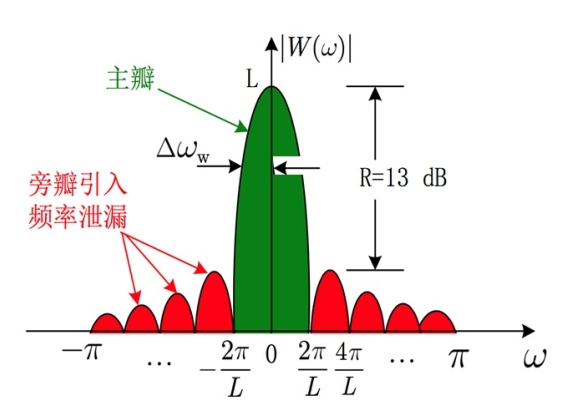
\includegraphics[width=0.6\textwidth]{chap3/img/DTFT_window.png}
        \caption{窗函数的频谱}
        \label{fig:DTFT_window.png}
    \end{figure}
    为方便起见,我们定义它的\bd{主瓣宽度}为
    \begin{align*}
        \Delta\omega_W = \frac{2\pi}{L}.
    \end{align*}
\end{example}

\subsubsection{频谱分辨率}

\begin{example}
    给定信号
    \begin{align*}
        x(n) = A_1\mathe^{\mathi\omega_1 n} + A_2\mathe^{\mathi\omega_2 n},
    \end{align*}
    其中 $n \in \set{Z}, 0 < \omega_1 < \omega_2 < \pi$,
    在一个奈奎斯特区间内,它的 DTFT 为
    \begin{align*}
        X(\omega) = 2\pi(A_1\delta(\omega - \omega_1) + A_2\delta(\omega - \omega_2)).
    \end{align*}
    画出它的频谱如 \ref{fig:DTFT_two_freqs.png} 所示。
    \begin{figure}[H]
        \centering
        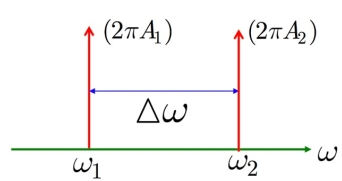
\includegraphics[width=0.3\textwidth]{chap3/img/DTFT_two_freqs.png}
        \caption{两个频率的信号的频谱}
        \label{fig:DTFT_two_freqs.png}
    \end{figure}
    可以看出,这两个频率的间隔为 $\Delta\omega = \omega_2 - \omega_1$。
\end{example}

\begin{example}
    给定信号
    \begin{align*}
        x_L(n) = A_1\mathe^{\mathi\omega_1 n} + A_2\mathe^{\mathi\omega_2 n},
    \end{align*}
    其中 $n \in [0, L-1], 0 < \omega_1 < \omega_2 < \pi$,
    在一个奈奎斯特区间内,它的 DTFT 为
    \begin{align*}
        X_L(\omega) & = \frac{1}{2\pi}X(\omega) \otimes W(\omega) \\
        & = A_1W(\omega - \omega_1) + A_2W(\omega - \omega_2).
    \end{align*}
    画出它的频谱如 \ref{fig:DTFT_two_freqs_window.png} 所示。
    \begin{figure}[H]
        \centering
        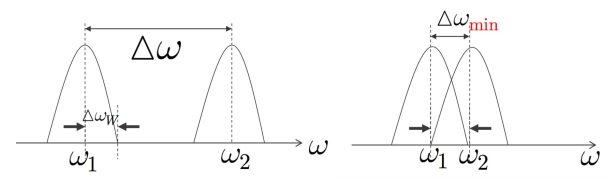
\includegraphics[width=0.6\textwidth]{chap3/img/DTFT_two_freqs_window.png}
        \caption{两个频率的信号的频谱}
        \label{fig:DTFT_two_freqs_window.png}
    \end{figure}
    可以看出,这两个频率的间隔为 $\Delta\omega = \omega_2 - \omega_1$。
\end{example}

\begin{definition}[频谱分辨率]
    那么当 $\Delta\omega$ 很小时,我们如何判断两个频率之间的距离呢?
    或者换而言之,要求分辨出这两个频率,$\Delta\omega$ 至少要多大呢?
    这就引出了\bd{频谱分辨率}的概念。

    当 $\Delta\omega$ 不小于窗函数的主瓣宽度 $\Delta\omega_W = 2\pi/L$ 时,
    我们认为可以分辨出两个频率。也就是说,定义 DTFT 的\bd{频谱分辨率}为
    \begin{align*}
        \Delta\omega_{\min} = \Delta\omega_W = \frac{2\pi}{L},
    \end{align*}
    其中 $L$ 是窗函数的宽度(即序列的长度)。
\end{definition}

\begin{remark}
    序列加窗后会对频谱产生两种影响:
    \begin{enumerate}
        \item 序列频谱中可分辨的最小频率间隔由数据长度决定,
            即窗函数的时间长度。这个现象被称为\bd{不确定原理}。
        \item 序列频谱中出现了高频分量。它们是由于矩形窗
            两个边缘处的突变所造成的。这个现象被称为\bd{频率泄漏}。
            好像是这些原来谱中没有的高频成分是从``内部''(信号原谱分布区间)中
            ``泄漏''出来的一样。显然,这些泄漏量与窗函数的旁瓣有关系,如
            图 \ref{fig:DTFT_leakage.png} 所示。
            \begin{figure}[H]
                \centering
                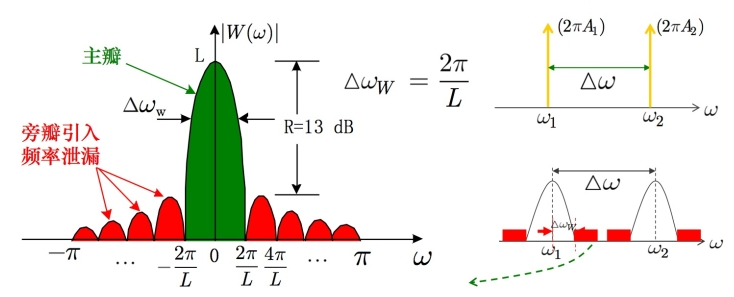
\includegraphics[width=0.6\textwidth]{chap3/img/DTFT_leakage.png}
                \caption{频率泄漏}
                \label{fig:DTFT_leakage.png}
            \end{figure}
    \end{enumerate}
\end{remark}
